%\documentclass[a4paper,10pt]{article}
\documentclass[
a4paper,
fleqn,
DIV=15,
pagesize
]{scrartcl}
\usepackage{color}
\usepackage{subfigure}
\usepackage{booktabs}
\usepackage{enumitem}
\usepackage{graphicx}
\usepackage[utf8]{inputenc}
\usepackage{hyperref}

\graphicspath{{eps/},{../plot/}}

%\setlength{\parindent}{0pt}

\begin{document}
\subject{MBSim -- Environment}
\title{MBSimGUI}
\subtitle{First Steps}
\author{Martin Förg}
\date{09.09.2020}

\maketitle

\begin{abstract}
This document shows first steps using the multibody simulation software
\textsc{MBSimGUI}. After installation and start a
simple model of a free falling body will be set up and simulated. Finally, it is shown how to load one of the existing model examples that are available on \textsc{GitHub}.
\end{abstract}

%\cleardoublepage

\tableofcontents

%\cleardoublepage

\section{Installation} \label{installation}
Download the latest release from
\url{https://www.mbsim-env.de/service/releases} and extract it to a folder of
your choice. \textsc{MBSimGUI} is now ready to use. If you want to integrate
\textsc{MBSimGUI} in your desktop environment, e.\,g. to have a shortcut on
your desktop, descend to the \emph{bin} folder and execute the script
\emph{desktopIntegration}\footnote{There are two files named
\emph{desktopIntegration} in this folder, one for \textsc{Linux}
(*.\emph{sh}) and one for \textsc{Windows} (\emph{*.bat}).}.

\section{Starting the GUI}

If you have run \emph{desktopIntegration} in chapter \ref{installation}, just double-click on \textsc{MBSimGUI} on your desktop. Otherwise, change to the \emph{bin} folder and start the application from there.

Starting \textsc{MBSimGUI} opens a new window, the main window, as shown in figure \ref{GUI}.
\begin{figure}
\centering
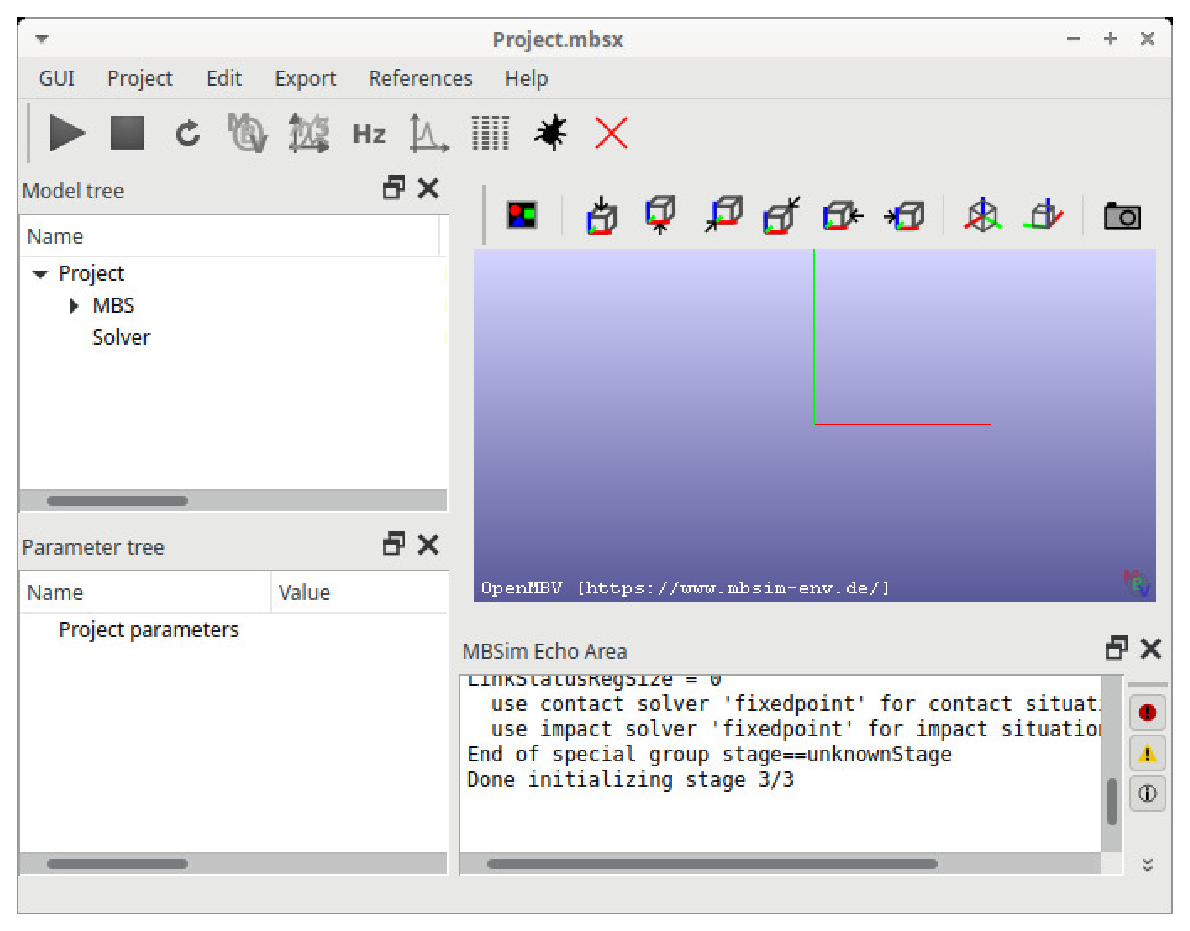
\includegraphics[scale=0.4]{GUI}
\caption{The GUI.} \label{GUI}
\end{figure}
The main window provides the following widgets:
\begin{itemize}
  \item the menu bar on top of the window allows for setting GUI options, managing
  projects and exporting project data.
  \item the buttons bar provides buttons to start and stop the simulation, to open
  the animation or the plotting tool and to debug the model.
  \item the model tree contains all elements of the project in particular the multi-body system (MBS) and its elements as well as the solver.
  It allows for adding and removing elements as well as setting their properties. Moreover, the solver element offers different numerical solvers like integrators or
  linear system analyzers.
  \item the parameter tree contains all parameters associated with the project or one of its elements. It allows for adding and removing parameters as well as setting their properties.
  \item the 3D view shows the model in terms of the design of its elements. The view on the MBS can be translated, rotated and zoomed.
  \item the echo area gives some informations to the simulation process and shows possible model errors.
\end{itemize}

Whenever we begin a new project there is already one element existing within the MBS. It is the inertial frame named
"I" which is always the starting point of your modeling. All absolute values to
be defined or calculated are related to this frame. The different colors refer
to the axes {\color{red} x}, {\color{green} y} and {\color{blue} z} of the
coordinate system.

To change the view on the MBS you can use one of the standard view buttons or
just press one of the three mouse buttons while moving the mouse within the 3D
view. For rotation use the left, for translation the right and for zoom the
middle mouse button.

\section{A simple example}
Now we are going to simulate a free fall of a rigid body. By default gravitation is enabled
acting along the negative {\color{green}y-axis}.

First, we will add a rigid body with a DOF along the {\color{green}y-axis}. For this,
open the elements "Project" and "MBS" in the model tree. In order to open an
element within the tree just left-click on the arrow next to the element.
A right-click on the container named "objects" shows a context menu. From there
choose "Add body" and then "Add rigid body".

A properties dialog opens for setting the body's data. Go to the tab named
"Kinematics", activate "Translation" and choose "Translation along y axis" from
the drop down list (figure \ref{rigidbody:prop}). Press the "OK" button to
apply the change and to close the dialog. In the 3D view a blue body should
appear (figure \ref{rigidbody:view}).
\begin{figure}
\centering
\subfigure[Property dialog of the rigid body.]{
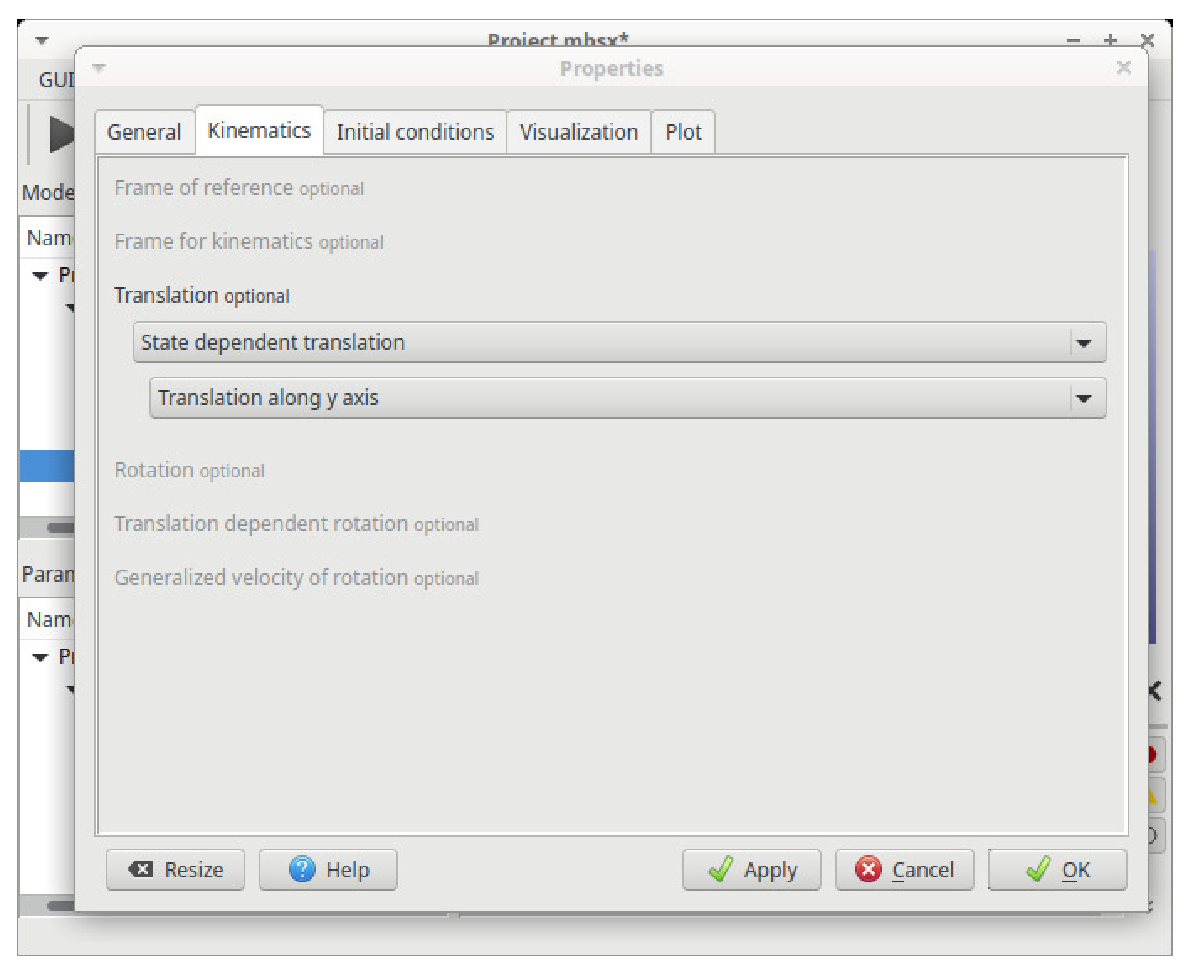
\includegraphics[scale=0.4]{kinematics} \label{rigidbody:prop}
}
\subfigure[3D view of the rigid body.]{
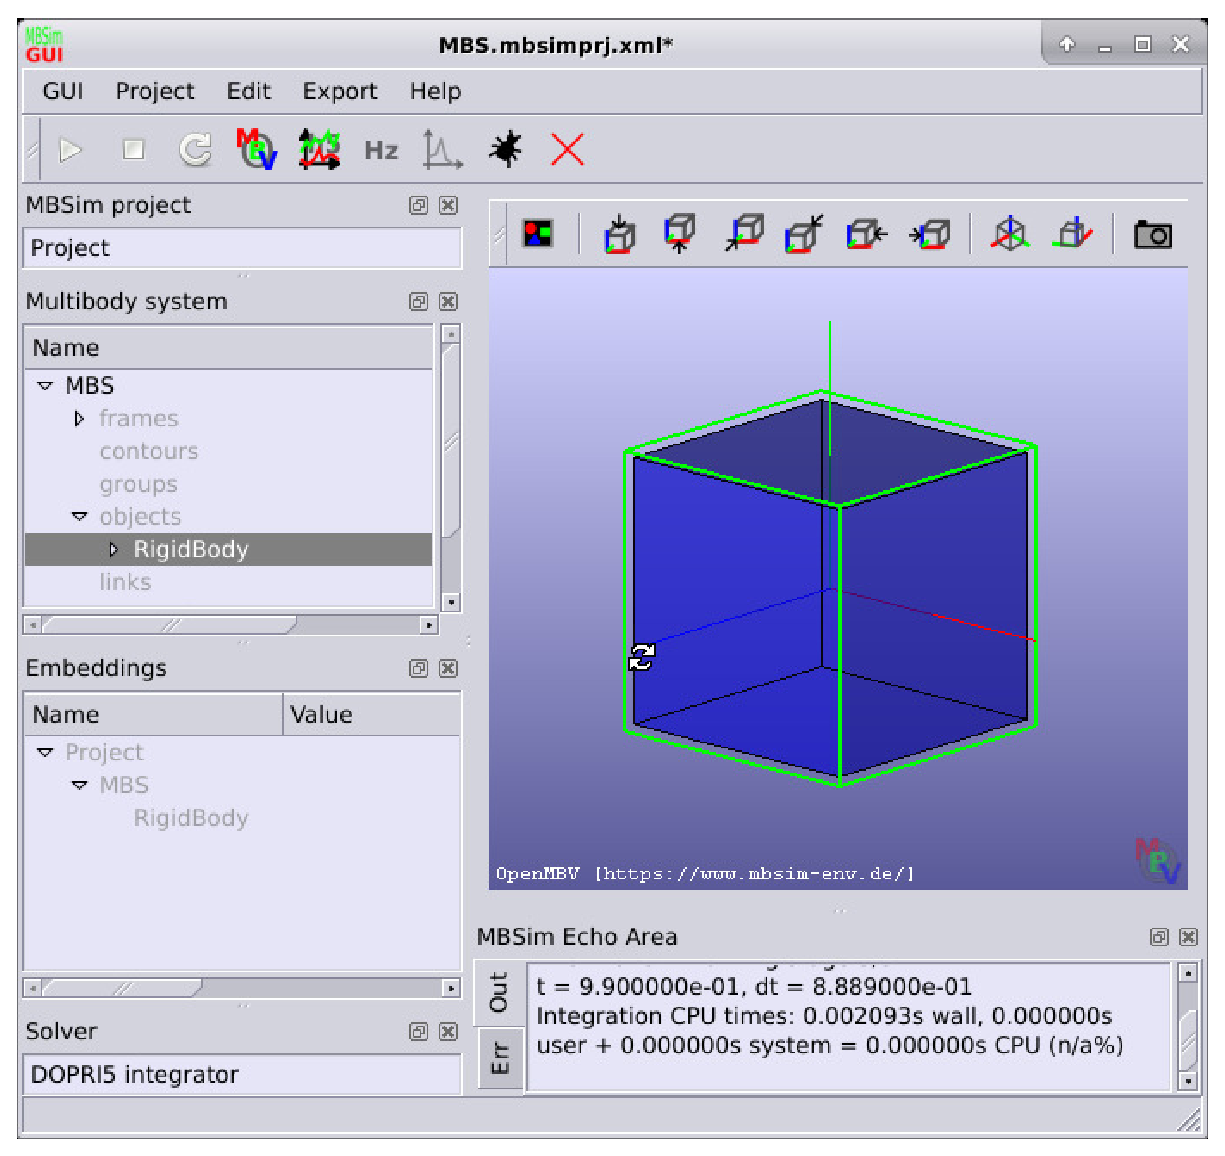
\includegraphics[scale=0.4]{body} \label{rigidbody:view}
}
\caption{Adding a rigid body to the MBS.} \label{rigidbody}
\end{figure}

Now, push the "Start simulation" button, which is the most left button in the
buttons bar. After the simulation is finished we can animate the body's
motion using \textsc{OpenMBV}.

Push the "OpenMBV" button in the middle of the buttons bar to start
\textsc{OpenMBV}.
\begin{figure}
\centering
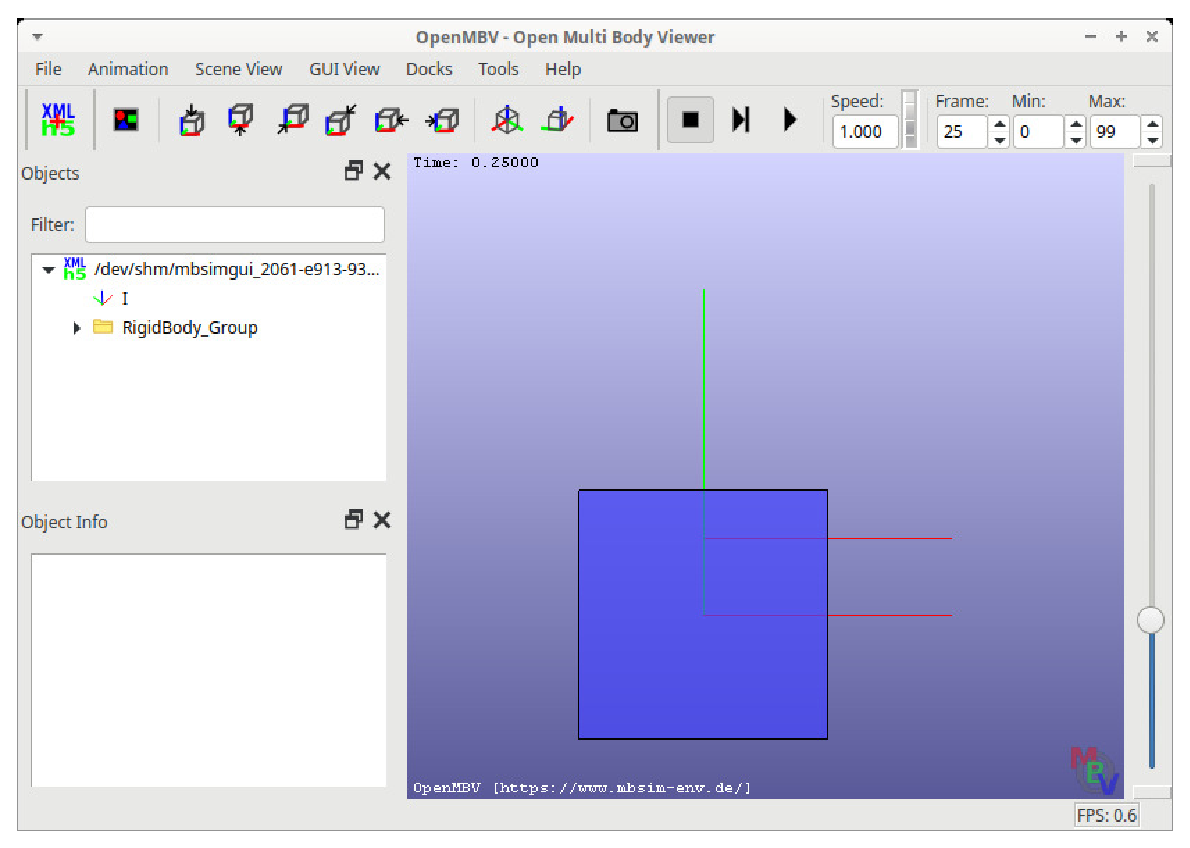
\includegraphics[scale=0.4]{openmbv}
\caption{The animation tool \textsc{OpenMBV}.} \label{openmbv}
\end{figure}
For animation click
the most right button in the buttons bar named "Run". We see the body falling
along the {\color{green}y-axis} of the inertial coordinate system (figure
\ref{openmbv}).

\section{Loading an existing model example}

\begin{figure}
\centering
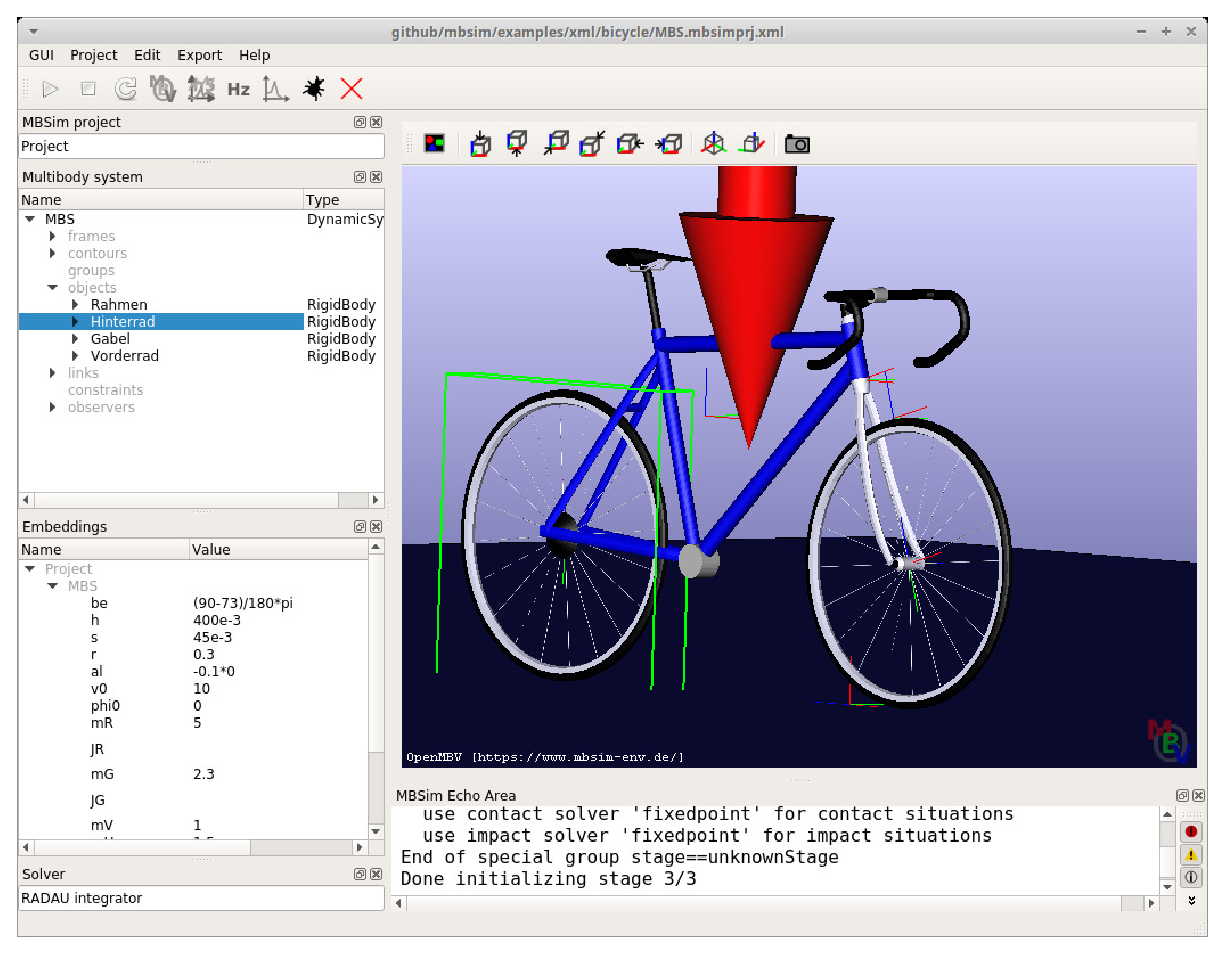
\includegraphics[scale=0.4]{bicycle}
\caption{Model of a controlled bicycle.} \label{bicycle}
\end{figure}
There are numerous model examples that demonstrate the features and capabilities of \textsc{MBSim}. Just visit the \textsc{GitHub} repository at \url{https://github.com/mbsim-env/mbsim} and step into \emph{examples/xml} to get an overview of the existing projects that can be loaded by \textsc{MBSimGUI}. The folder \emph{bicycle} for example contains a model of a controlled bicycle, see figure \ref{bicycle}.

The project files can be downloaded separately or at once by dowloading the complete \textsc{MBSim} source archiv \url{https://github.com/mbsim-env/mbsim/archive/master.zip}. To load a specific model just click "load" in "Project" menu and select the corresponding project file with the extension \emph{*.mbsx}.

\end{document}
